\section{Experiments}
\label{sec:exps}

In this section we report on our preliminary experiments conducted with the prototype tool
whose implementation has been described in \Cref{sec:impl}. All these experiments can be
easily reproduced by downloading our project at \url{http://www.disi.unige.it/person/AnconaD/\toolName}.

Since one of the main use of Node.js is the development of Web applications,
we have focused on runtime verification of code based on the \lstinline{http} module.

First, the documentation of the module\footnote{Available at \url{https://nodejs.org/api/http.html}.} has been inspected  
with the purpose of mining specifications of the features provided by \lstinline{http}.
Several of them can be easily translated in corresponding trace expressions
that have been employed in our tool to automatically monitor correct use of the \lstinline{http}
module by client code.

Six constraints that are not enforced by the library have been identified on the use of the functions exported by \lstinline{http};
correspondingly, six trace expressions have been derived to
dynamically check such constraints and detect the related bugs.
In each trace expression we use the filter operator to restrict the event domain to functions that are relevant for the specification.

The tool has been tested in two different ways.
At a first stage, simple server and client Node.js applications based on \lstinline{http} have been developed,
and violations of the module specifications have been deliberately introduced in the code,
to verify that the tool is effectively able to detect illegal use of the \lstinline{http} features.

Then, at a second stage, the tool has been experimented with real and widely used code based on  \lstinline{http}.
To this aim, the Web application framework Express\footnote{See \url{https://expressjs.com/}.} has been
selected for our test: it offers a large number of HTTP utility methods and middleware functions for more rapid, efficient
and robust development of HTTP APIs, and, for these reasons, several popular Node.js frameworks and Node.js Web applications
are built on top of it. 

\subsection{Mining Specifications from the \lstinline{http} Module Documentation}\label{sec:spec-minining}

The documentation of the standard Node.js \lstinline{http} module has been carefully inspected to find illegal uses
of the provided features.
As an example, \Cref{fig:httpDoc} shows an excerpt concerning \lstinline{http.ClientRequest};
objects are internally created with this constructor and returned from \lstinline{http.request()}.
\begin{figure}
	\framebox{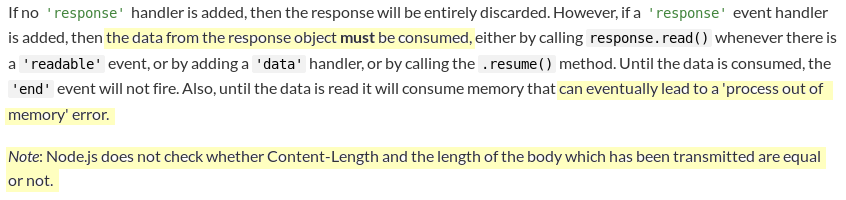
\includegraphics[width=\textwidth]{fig/httpExcerptHighlight}}
	\caption{Excerpt from the \lstinline{http} documentation at \url{https://nodejs.org/api/http.html}.}
	\label{fig:httpDoc}
\end{figure}
The highlighted sentences reveal two possible issues:
\begin{itemize}
\item \textbf{unconsumed data}: in case the client defines a handler for the server response, data from the response must be consumed,
  otherwise a `process out of memory' error can occur;
\item \textbf{content length}: unchecked length of the body of a request/response can block the communication, or data can be lost, as already shown
  in \Cref{sec:web-req}.
\end{itemize}
In the first case, the correct behavior can be captured by the following trace expression $\tau$ defined as follows:
\begin{align*}
\tau &= \var{id}{\onData(\avar{id}) \prefixop ((\onEnd(\avar{id}) \prefixop \emptyseq) \shuffleop \tau)}
\end{align*}
where the variable $\avar{id}$ corresponds to the id of the specific response, whereas the event types
$\onData$ and $\onEnd$ capture the handling of the \lstinline{'data'} and \lstinline{'end'} events, respectively.
As shown in previous examples, combination of shuffle and recursion is essential to be able to deal with
an arbitrary number of different responses which can be received by a client.

In the second case, the trace expression which is used for checking the correct behavior of code dealing with
\lstinline{http.ClientRequest} objects has already been presented in \Cref{sec:web-req}.

Besides the two properties discussed above, the following four additional specifications have been mined from
the documentation and expressed with corresponding trace expressions:
\begin{itemize}
\item \textbf{omitted body}: depending on the request received by the client or the response sent by the server, there are cases when the response must not
  contain a body, hence
  a server which tries to include a body in such situations does not behave correctly. The different cases require
  different treatments and trace expressions, as follows:
  \begin{itemize}
  \item \textbf{HEAD request}: when the method of the request sent by the client is HEAD;
  \item \textbf{204 response}: when the response of the server has status code 204 (no content);
  \item \textbf{304 response}: when the method of the request sent by the client is a conditional GET and access is allowed, and the response
    server has status code 304 (not modified) because the requested document has not been modified.
  \end{itemize}
\item \textbf{write head}: the method \lstinline{writeHead} to write the head of a server response must only be called once on a message and it must happen before
  the method \lstinline{end} is called to signal to the server that the response is complete. If this rule is not followed, then
  a default header, most likely different from the intended one, is written in the response.
\end{itemize}
While some of the mined specifications directly depend from the specific implementation of \lstinline{http}, others
are more related to the specification of the HTTP protocol; indeed, other trace expressions could be mined by looking at the
standard specification of HTTP, to dynamically check that a server (resp. client) implementation in Node.js verifies the HTTP
requirements.

\subsection{Testing the Tool with Simple Applications}
\label{sec:simple-test}
The tool has been tested with the trace expressions of the specifications presented in the previous section by performing
runtime verification of simple servers/clients implemented in Node.js.
For all specifications both correct and incorrect code has been developed, to verify the absence of both false negatives and positives.

Consider for instance the last specification presented in \Cref{sec:spec-minining}: 
the header of a server response must be written before calling the \lstinline{end} method which finalizes the response.

A very simple server verifying the specification is the following one:
\begin{lstlisting}
const http = require('http');

const server = http.createServer((req, res) => {
	// preparing response...
	res.writeHead(200);
	res.end(() => console.log('response sent'));
});

server.listen(80);
\end{lstlisting}

As expected, in this case the tool does not report any anomalous behavior.
However, if we modify the code above as follows
\begin{lstlisting}
const http = require('http');

const server = http.createServer((req, res) => {;
	res.end(() => console.log('response sent'));
	// BUG! writing header after calling end() method
	res.writeHead(204);
});

server.listen(80);
\end{lstlisting}
and monitor the server with our tool, then we get an error message associated with the following event, corresponding
to a call to \lstinline{writeHead}:
\begin{lstlisting}
{ event: 'func_pre',
  name: 'writeHead',
  id: 12,
  res: undefined,
  args: [ 204 ],
  targetId: 10,
  resultId: undefined }
\end{lstlisting}

Similar examples have been used to test our tool with the other specifications.

\subsection{Testing the Tool with Express}\label{sec:express}

After the simple experiments conducted in the first phase as described in the previous section,
a natural next step towards the assessment of our tool consisted in testing popular real Node.js code
based on \lstinline{http}.
% to do that, we have considered Express\footnote{See \url{https://expressjs.com/}.}, a very (if not the most) popular framework based on \lstinline{http} to develop Node.js web applications.

To this aim, the three components of Express depending on \lstinline{http} (\lstinline{application.js}, \lstinline{request.js} and
\lstinline{response.js}) have been instrumented with Jalangi2, for a total of almost 1K SLOC.
As for the other tests of \Cref{sec:simple-test}, we have reused the same Jalangi2 instrumentation and trace expressions defined in \Cref{sec:spec-minining}.

Then the use of \lstinline{http} by Express has been dynamically monitored with our tool through simple
examples of server applications written with Express as the following one:
\begin{lstlisting}
const express = require('express');
const morgan = require('morgan');
const responseTime = require('response-time');
const serveIndex = require('serve-index');

const path = process.cwd();
const app = express();

app.use(morgan('combined'));
app.use(responseTime());
app.use('/', express.static(path), serveIndex(path, {'icons': true}));
app.get('/*', (req, res) => {
    res.writeHead(404, {'Content-Type': 'text/html'});
    res.end('Not found\n');
});

app.listen(80);
\end{lstlisting}
Although the application contains only a dozen of source lines of code, the
functionalities of the server are not so trivial, thanks to Express and the
associated middleware \lstinline{morgan}, \lstinline{response-time}, \lstinline{serve-static} and
\lstinline{serve-index}.

The \lstinline{morgan} module creates a logger middleware function that allows the server to log (on the standard output, in this example)
information about the received requests, while the \lstinline{response-time} module
creates a middleware that records the response time of the HTTP server, that is, the elapsed time from when a
request enters the middleware to when the headers are written out to the client.

The  \lstinline{serve-static} middleware serves files from within a given root directory (in this case, the same directory
from which the server has been launched), while \lstinline{serve-index} serves an index (with displayed icons in this case)
of the directory of the server based off the URL value of the request. In practice, the server allows inspection of the directory
from which it has been launched, included all its subdirectories, and downloading of all files rooted at it. 

Finally, the last call \lstinline{app.get} deals with the case when no directory or file could be found.
The tool has been tested with the server above, and a Node.js client sending requests with random  paths based on its root directory at the frequency of three requests per second.
The tool was able to monitor all relevant \lstinline{http} events triggered in the above mentioned Express components used through the server, showing that our instrumentation and monitoring system can deal with code bases of considerable size using all the main features of the programming language.
As expected, though, Express it is correct w.r.t.\ the previously described constraints on the use of the \lstinline{http} module.

\subsection{Benchmarks}

All tests presented in Section~\ref{sec:spec-minining} have been employed as benchmarks for performance evaluation
of our prototype on an Intel(R) Core(TM) i7-6500U CPU at 2.50GHz with a 16GB RAM, running SWI-Prolog 7.2.3 on
Linux kernel 4.14.40.
In particular, we have measured how much the performances of all implemented servers are affected by runtime monitoring;
only correct implementations have been considered, to be able to overload servers with arbitrary numbers of requests.
The benchmarks have shown that the overhead of runtime verification is mainly due to code instrumentation, rather than the particular monitored
specification, therefore all measurements have been conducted while verifying the same trace expression, namely, 
the one corresponding to the specification \textbf{omitted body (204 response)}.

Table~\ref{table} shows the results of our experiments. 
\begin{table}[ht]
  \begin{tabular}{|l|l|l|l|}
    \hline
    \textbf{Benchmark} & 
    \textbf{Original} &
    \textbf{Monitored} &
    \textbf{Overhead} \\
    \hline
    \multicolumn{4}{|c|}{HTTP module}\\
    \hline
    Content length & 
    591 RPS &
    528 RPS &
    12 \% \\

    Omitted body (HEAD request)&
    631 RPS &
    588 RSP &
    7 \% \\

    Omitted body (204 response)&
    638 RPS &
    626 RSP &
    2 \% \\

    Omitted body (304 response)&
    634 RPS &
    626 RSP &
    1 \% \\

    Unconsumed data &
    643 RPS &
    739 RPS &
    -13 \% \\

    Write head &
    627 RPS &
    580 RPS &
    8 \% \\
    \hline

    \multicolumn{4}{|c|}{Express}\\
    \hline
    Hello world & 
    766 RPS &
    716 RPS &
    7 \% \\

    File explorer &
    588 RPS &
    312 RPS &
    88 \%\\

    \hline
  \end{tabular}
  \caption{Benchmark results}
  \label{table}
\end{table}
For each benchmark we have measured the average number of served requests per second (RPS) 
with a client running a loop to continuously send requests to the server without waiting to collect its response;
all measurements have been obtained as the average over ten different runs, each consisting
of 100K requests sent to the server.

The second column (Original) displays the values concerning the original server, while the third one
(Monitored) reports the measurements for the same server under monitoring.
For all simple servers directly implemented with the \lstinline{http} module we registered modest overheads, as well
as for the Express server sending the response \lstinline{'Hello world'} to all requests.
Interestingly, the monitored version of \textbf{unconsumed data} outperforms the original version; we have
not investigated yet the reasons of such a behavior.

For the file explorer built with Express and presented in Section~\ref{sec:express}, the client keeps sending GET requests
with randomly generated paths; in this case the overhead is more significant, but still the overall performance 
is acceptable: the server could operate at the rate of more than 300 RPS, while the system had to monitor more than 1.5 million events.
Such a result shows that the optimizations introduced in our prototype implementation allowed us
to get a 100x speed boost, and that runtime monitoring can be effectively employed for testing servers implemented with Express.

